\documentclass[titlepage]{article}
\usepackage[utf8]{inputenc}
\usepackage[a4paper, total={16cm, 23cm}, top=3.5cm]{geometry}
\usepackage[dvipsnames]{xcolor}
\definecolor{linkcolor}{RGB}{51, 54, 142}
\usepackage{
    amsmath,
    amssymb,
    amsthm,
    fancyhdr,
    siunitx,
    bm,
    lipsum,
    standalone,
    tikz,
    booktabs,
    enumitem,
    array,
}
\usepackage[colorlinks=true, allcolors=linkcolor]{hyperref}
\usepackage[
    backend=biber,
    bibstyle=ext-authoryear,
    citestyle=ext-authoryear-comp,
    sorting=nyt,
    uniquename=false,
    maxbibnames=99,
    giveninits=true,
]{biblatex}
\DeclareFieldFormat[article]{volume}{\mkbibbold{#1}}
\DeclareFieldFormat[article]{number}{\mkbibparens{#1}}
\DeclareFieldFormat[article]{pages}{#1}
\renewcommand*{\volnumdelim}{}
\renewbibmacro{in:}{}
\addbibresource{references.bib}

\pagestyle{fancy}
\fancyhead{}
\rhead{Research Proposal}
\renewcommand{\headrulewidth}{0.5pt}

\setlength{\headheight}{15pt}
\setlength\parindent{0pt}
\setlength\parskip{6pt}

\renewcommand{\d}[1]{\mathrm{d}#1}
\newcommand{\diff}[2]{\frac{\mathrm{d} #1}{\mathrm{d} #2}}
\newcommand{\ddiff}[2]{\frac{\mathrm{d}^2 #1}{\mathrm{d} {#2}^2}}
\newcommand{\pdiff}[2]{\frac{\partial #1}{\partial #2}}
\renewcommand\vec{\bm}
\newcommand{\uvec}[1]{\vec{\hat{#1}}}

\def\equationautorefname~#1\null{%
    (#1)\null
}
\newcommand{\rb}{Rayleigh-B\'{e}nard}
\newcommand{\prandtl}{\ensuremath{\mathrm{Pr}}}

\begin{document}
\begin{titlepage}
\begin{center}
    {\Huge \textbf{%
        Towards transparent data-driven parametrisations for weather and
        climate modelling
    }} \\
    \vspace{0.75cm}
    {\Large\textbf{Honours Research Project Proposal}} \\
    \vspace{0.75cm}
    {\Large\textbf{Thomas D. Schanzer}} \\
    \vspace{6pt}
    {\large Supervisor: Prof. Steven Sherwood} \\
    \vspace{0.75cm}
    {\large%
        School of Physics

        Climate Change Research Centre and
        ARC Centre of Excellence for Climate Extremes

        University of New South Wales, Sydney, Australia
    }
\end{center}
\vfill
\begin{center}
{\large\textbf{Abstract}}

\begin{minipage}{13cm}
    Constrained by computational resources, numerical models of Earth's
    atmosphere and oceans are unable to resolve important fine-scale dynamical
    features. The effect of the unresolved behaviour on the coarse state of the
    models must be estimated in a process known as parametrisation, but
    deficiencies in traditional parametrisation schemes inhibit accurate
    forecasting and climate prediction. The proposal for this Honours project
    is to help bridge the gap between parametrisation methods that have shown
    promise in simple toy models and the ultimate goal of generalising them to
    produce rigorous, accurate, robust and transparent schemes in full-scale
    Earth models. More specifically, the project aims to parametrise the
    subgrid-scale dynamics of 2D \rb{} convection, an intermediate-complexity
    fluid problem, using promising methods from toy model research. By
    evaluating the performance of these schemes, the project will identify
    their strengths and weaknesses and determine how well they generalise to
    more complex models.
\end{minipage}
\end{center}
\vfill
\renewcommand{\baselinestretch}{0.75}\normalsize
\tableofcontents
\renewcommand{\baselinestretch}{1.0}\normalsize
\end{titlepage}

\newpage
\pagestyle{fancy}
\thispagestyle{fancy}
\section{Introduction}
\subsection{Background}
% how do earth system models work? what do they do? why do we need them?
The Earth system (including atmosphere, ocean and land) is distinguished both
in its complexity and its influence on all terrestrial life. If the wellbeing
of humanity in particular is to be preserved, it is difficult to overstate the
importance of understanding and predicting this system's behaviour---both
short-term weather and long-term climate. This understanding and predictive
skill informs important decisions and government policies that have the
potential to reduce our vulnerability to extreme events (e.g., floods,
droughts, fires, tropical cyclones) and long-term climate change, and limit
negative human impacts (e.g., greenhouse gas emissions) to sustainable levels.

A significant part of our understanding and predictive skill is derived from
numerical modelling of the Earth system. Like many other models, the aim is to
predict the time evolution of an initial state (e.g., pressure, temperature,
wind velocity in the atmosphere) given a set of boundary conditions and
external forcings.
% what makes modelling hard? why do we need parametrisation?
Unfortunately, there are many obstacles to accurate modelling. Arguably the
most fundamental of these is chaos: even with a perfect model and unlimited
computing resources, arbitrarily small differences in initial conditions
grow exponentially. This constrains short-term predictability. Second,
the Earth system comprises a vast number of interacting components, such as
water in all three phases, solar radiation and clouds (just to name a few which
are relevant to atmospheric modelling). In other words, the system is
high-dimensional. Third, the dynamics occur on a wide spectrum of spatial
and temporal scales. These range from large-scale, slowly-evolving motions
such as ocean gyres and the atmospheric Hadley circulation, to synoptic-scale,
transient weather systems and ocean eddies, to
small-scale wind gusts, tornadoes, water waves and turbulence. All scales
and their cross-interactions influence the overall dynamics.

Atmosphere and ocean models solve the differential equations that govern fluid
flow with a finite spatial and temporal resolution and are therefore only able
to resolve behaviour whose scale is of the same order of magnitude as the
resolution or larger. The achievable resolution is constrained by the
capabilities, availability and cost of modern computing resources. A typical
atmospheric global climate model has a spatial resolution on the order of
$\ang{1}$ latitude/longitude, roughly corresponding to the size of the entire
Greater Sydney area from Katoomba to Bondi. Sub-grid scale features, such as
individual clouds, cannot be explicitly resolved, but to ignore them completely
would introduce unacceptable biases (inaccuracies, relative to observations)
in the model output. % ref?
The same is true for the numerous components of the Earth system that influence
the fluid dynamics but are not directly predicted by the fluid equations, such
as solar radiation and land interactions (which include moisture and heat
fluxes from vegetation, soil and water bodies).

% how has parametrisation been done historically?
The process of using the information available in the model to estimate the
effect of these unresolved processes on the coarse-scale variables is known as
\emph{parametrisation}, which will be the topic of the project. A general
mathematical picture of parametrisation can be developed by considering a
system with some degrees of freedom ``hidden'' from the observer, not
resolvable by the model. In general, the evolution of the resolvable and
unresolvable degrees of freedom is governed by a set of coupled PDEs with the
generic form
\begin{subequations} \label{eqn:coupled_system}
\begin{align}
    \label{eqn:resolved}
    \partial_t (\text{resolved variable})
        &= S_\mathrm{r}(\text{resolved variables})
        + C_\mathrm{r}(\text{unresolved variables}) \\
    \label{eqn:unresolved}
    \partial_t (\text{unresolved variable})
        &= S_\mathrm{u}(\text{unresolved variables})
        + C_\mathrm{u}(\text{resolved variables})
\end{align}
\end{subequations}
where $S_\mathrm{r},S_\mathrm{u},C_\mathrm{r},C_\mathrm{u}$ are (possibly
nonlinear) operators containing spatial derivatives. The $S$ terms are
self-interactions: the influences of the resolved and unresolved variables on
themselves. The $C$ terms are couplings: the influence of the resolved
behaviour on the unresolved behaviour and vice versa.

A model cannot solve \autoref{eqn:coupled_system} because it has no information
about the unresolved variables. The goal of parametrisation is to derive a
closed (i.e., well-posed) system involving only the resolved variables that
still yields an accurate solution for those variables. The model is thus
described by
\begin{equation} \label{eqn:model}
    \partial_t (\text{resolved variable})
        = S_\mathrm{r}(\text{resolved variables})
        + P(\text{resolved variables}),
\end{equation}
where $P$ is the \emph{parametrised tendency}: an estimate of the unseen
coupling term $C_\mathrm{r}$ in \autoref{eqn:resolved} based solely on the
values of the resolved variables. The study of parametrisation is essentially
concerned with the construction of the optimal $P$.

\subsection{Brief literature review}
Traditional parametrisations are often based on heavily simplified conceptual
models of the processes in question. For example, the well-known Community
Atmosphere Model v5 \parencite{cam5} parametrises atmospheric convection by
considering an ensemble of rising updraft plumes, making assumptions about
their mass flux and initiation conditions \parencite{zhang1995}.
% what are the limitations of traditional methods?
It is now known that many existing parametrisation schemes have biases that
do not reflect reality. For example, many precipitation schemes suffer from
the ``drizzle problem'': they overestimate the frequency of precipitation
and underestimate its intensity, failing to capture its variance and extreme
values \parencite{shamekh2022}. These biases limit the certainty of future
climate projections and our ability to understand how extreme precipitation,
for example, might change in the future.


% what work has been done to resolve these issues?
% how much success has there been?
% machine learning, continuous development, stochastic methods
A significant amount of work has been done to make parametrisation schemes more
rigorous and complete. A key development has been the introduction of
\emph{data-driven} techniques, which construct parametrisations by fitting
statistical models to a reliable dataset rather than primarily using
physically-motivated conceptual models. One of the most intensely studied
data-driven techniques in contemporary research is machine learning, typically
employing algorithms to ``learn'' how the sub-grid scale behaviour relates to
the resolved variables from high-resolution simulation data. For example,
\textcite{shamekh2022} trained an autoencoder on high-resolution precipitable
water data to produce a measure of convective organisation (the aggregation of
convective clouds). By training a neural network to predict this organisation
metric from the coarse-grid variables, they were able to capture the
statistical distribution of precipitation intensity, especially extremes, much
more accurately.

While parametrisation schemes are often tested in full-scale atmospheric
models---\emph{in situ}---the sheer scale of these models and the amount of
data they produce can make it difficult to understand where their strengths and
weaknesses lie. In particular, machine learning techniques, which have no basis
in physical intuition, are notoriously opaque (they are often called ``black
boxes''). For example, \textcite{shamekh2022} had to perform a rather detailed
analysis to prove that the output of their autoencoder was indeed a measure of
convective organisation. This has prompted some researchers to use very simple
toy models, rather than full atmospheric models, as test beds for the
construction and analysis of new, more transparent data-driven parametrisation
techniques. Another advantage of a simple model is that it can be solved with
high numerical precision, providing a reliable ``truth'' dataset for
data-driven techniques. In contrast, data-driven parametrisation for full
atmospheric models requires either observational data, which has inherent
uncertainties, or output from high-resolution simulations, which are not
perfect representations of the atmosphere either.

Two important parametrisation elements have been developed with the aid of toy
models. The first is stochasticity: the introduction of some randomness in the
parametrised tendencies to reflect the fact that the large-scale state does
not uniquely determine the fine-scale state. The second is memory: the dependence
of the parametrised tendency on its own value at previous times, or the values
of the resolved variables at previous times.

One of the seminal and most widely cited toy model parametrisation studies is
that of \textcite{wilks2005}. \citeauthor{wilks2005} used the so-called Lorenz
'96 model \parencite{lorenz1995}, which was devised by renowned meteorologist
Edward Lorenz. It matches the form of \autoref{eqn:coupled_system} by
construction, having a set of slowly-varying ``resolved'' variables coupled to
a larger set of rapidly-varying ``unresolved'' variables.
\citeauthor{wilks2005} first numerically solved the full coupled system as
``truth'' and used this data to retrospectively calculate the unresolved
tendencies ($C_\mathrm{r}$ in \autoref{eqn:resolved}). He then performed a
simple polynomial regression of the unresolved tendencies against the
resolved variables, as shown in \autoref{fig:wilks_regression} (a reproduction
of his Figure 2).

\begin{figure}
    \centering
    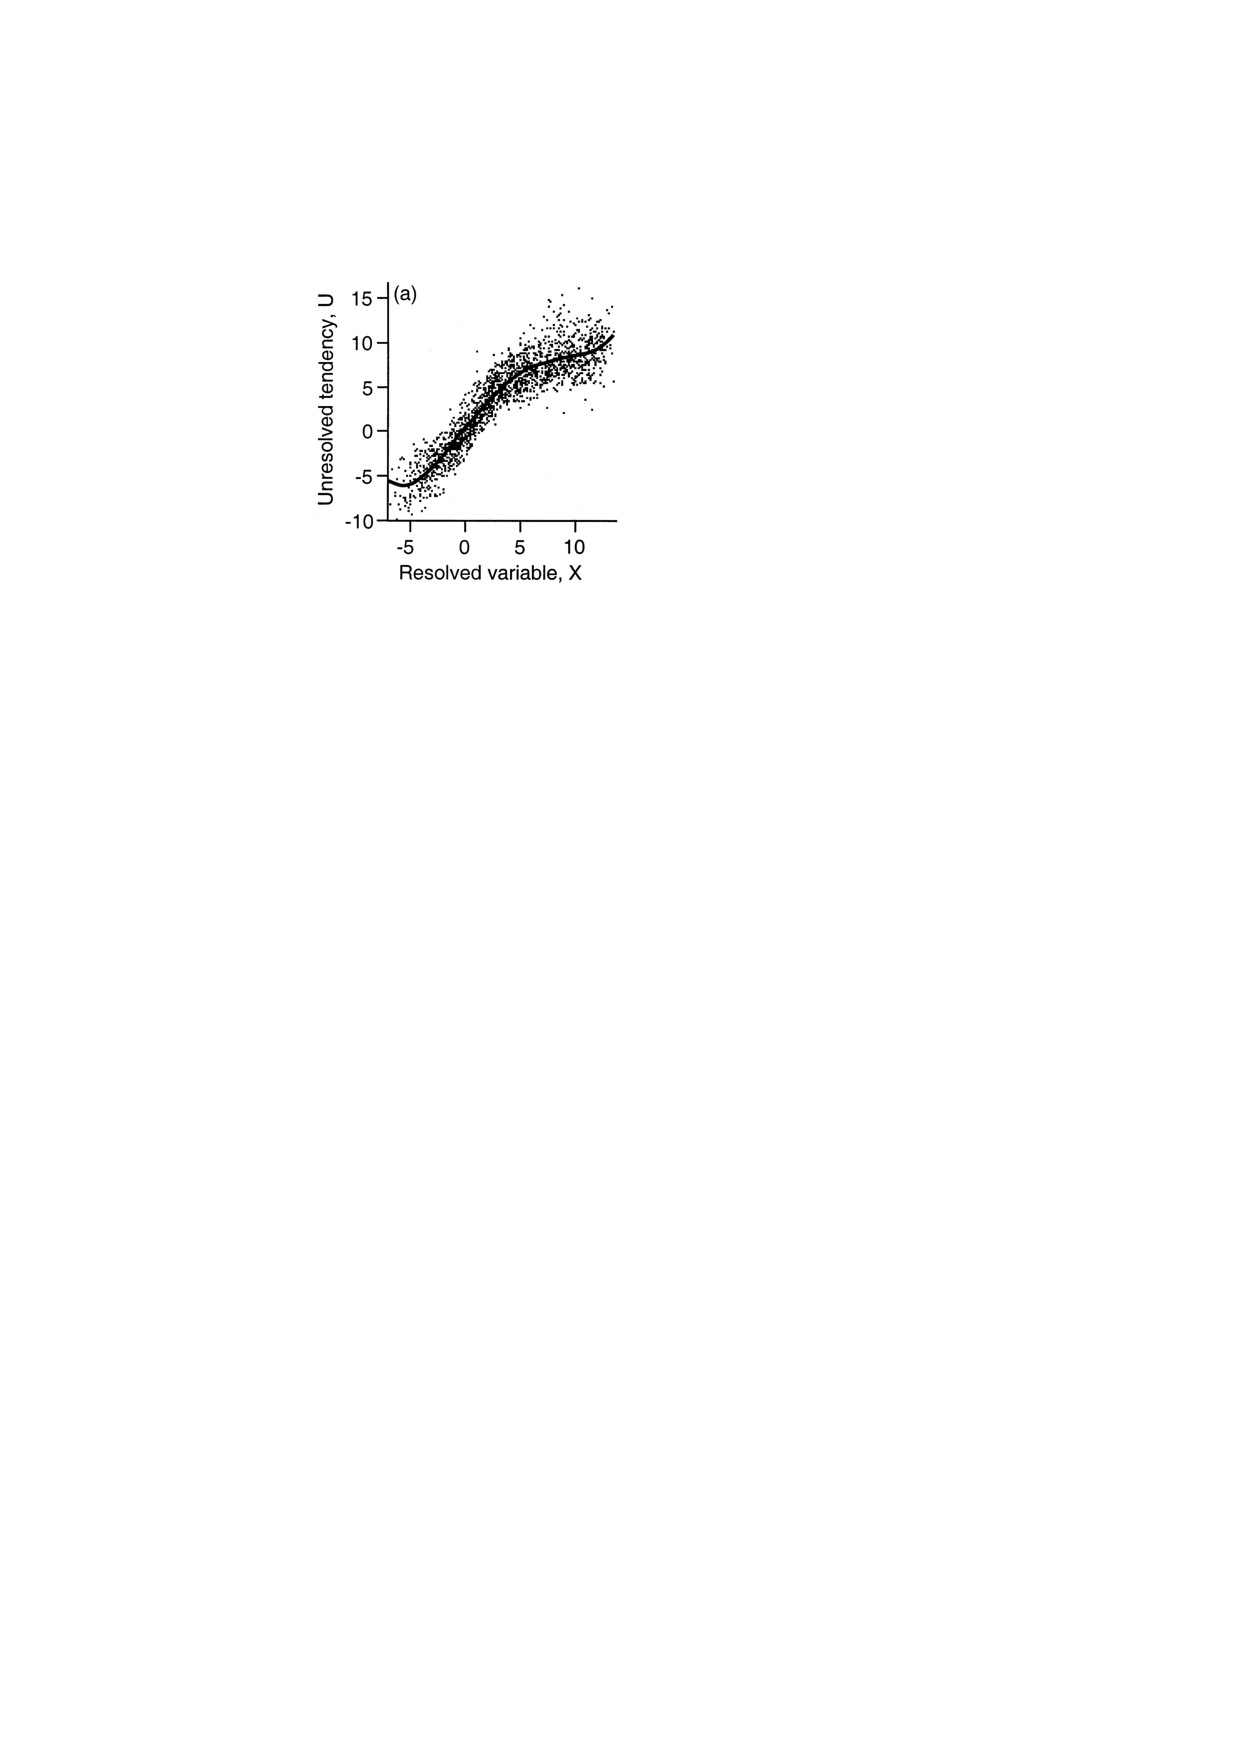
\includegraphics[width=0.35\linewidth]{figures/wilks_regression.pdf}
    \caption{
        A reproduction of Figure 2 by \textcite{wilks2005}, showing a
        scatter plot of the unresolved tendencies against the values of
        the resolved variables in the Lorenz '96 model, with the
        polynomial regression model plotted as a black line.
    }
    \label{fig:wilks_regression}
\end{figure}

\citeauthor{wilks2005} evaluated three parametrisation schemes. First, the
polynomial regression alone was used as a simple deterministic parametrisation
(i.e., the regression model was used as $P$ in \autoref{eqn:model}). The second
scheme added independent Gaussian (``white'') noise to the predictions of the
regression model in order to reflect the range of possible unresolved states
for a given resolved state (which manifests as a scatter around the curve in
\autoref{fig:wilks_regression}). The third scheme made the noise
non-independent by introducing non-zero \emph{temporal autocorrelation}; that
is, the value of the noise at time step $n$ is drawn from a Gaussian
distribution whose mean depends on the value of the noise at time step $n-1$.
This type of noise is ``red'', and such a scheme is technically known as a
first order autoregressive or AR(1) model. \citeauthor{wilks2005} found that
the third scheme (with both stochasticity and memory) was the most accurate in
reproducing the long-term average distributions of the resolved variables.

In the years following \citeauthor{wilks2005}' paper, other more sophisticated
parametrisation schemes have been tested. \textcite{crommelin2008}, for
example, implemented a stochastic scheme with memory based on conditional
Markov chains, also for the Lorenz '96 model. The Markov chain method assumes
that the unresolved tendencies can take only a finite set of values, or
``states'', with transitions between the states governed by a stochastic
process. The authors found that this scheme outperformed
\citeauthor{wilks2005}' AR(1) scheme in several respects. In summary, there
is clear agreement in the literature that memory and stochasticity should
be included in parametrisations.


\subsection{Proposed direction for research}
% what problems remain to be solved?
Despite the successes of toy model parametrisation studies, a common
shortcoming---and one that many authors have identified---is that they provide
limited information about how efficiently and effectively the techniques would
scale in real weather/climate models (e.g., \cite{wilks2005},
\cite{crommelin2008}).
% narrow it down: what problem will we solve?
This project aims to find a middle ground by testing parametrisation techniques
that have been shown to work in toy models on a more realistic model that
solves a real fluid problem.

% structural assumptions
Another consideration that seems to be unaddressed in the toy model literature
is the possibility for the dynamical system being modelled (e.g., the
atmosphere) to have \emph{inherent} stochasticity or memory, even before
parametrisation. These phenomena could arise if some degrees of freedom are
completely unknown to us, or if our physical understanding of the system is
incomplete (as is the case for the atmosphere). The project will therefore
also seek to determine the level of predictability that is achievable with
different parametrisation schemes under these circumstances.

\section{Proposed aims and methods}
\subsection{Chosen dynamical system}
This project will study parametrisation in the context of turbulent
two-dimensional \rb{} convection, which is the flow of a fluid between two
infinite flat plates of constant temperature, the bottom plate made warmer than
the top plate. This may be regarded as a simpler, more computationally
tractable analogue of true atmospheric convection whose fine-scale turbulent
behaviour will still be challenging to parametrise. While the (Navier-Stokes)
equations that govern the flow are omitted here, I will use a representation
where the dynamical variables are the vorticity $\omega$ (curl of the
velocity), temperature $T$ and streamfunction $\psi$ (a scalar function whose
level curves are streamlines of the flow). \autoref{fig:rbc} shows a typical
temperature plot for this type of flow.

\begin{figure}[ht]
    \centering
    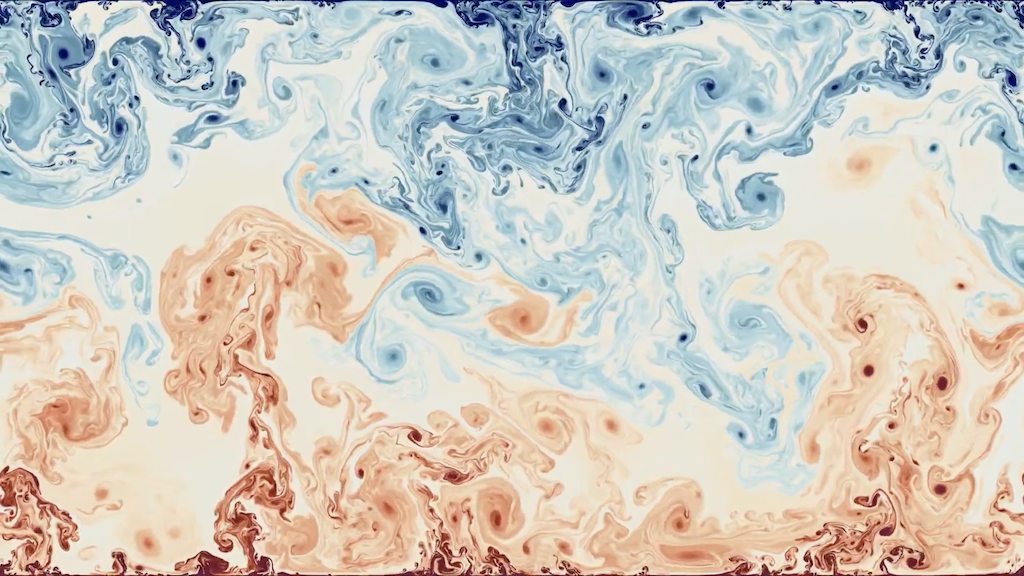
\includegraphics[width=0.7\linewidth]{figures/rbc.png}
    \caption{
        Temperature plot for a simulation of 2D \rb{} convection (red is hot,
        blue is cold). Courtesy of Stephan Lenz (2018), published on
        YouTube under the Creative Commons CC BY licence
        (\url{https://youtu.be/BJKiuwpdprQ}).
    }
    \label{fig:rbc}
\end{figure}

In its usual form, the system of PDEs for the flow does not distinguish
resolved dynamics from unresolved dynamics like \autoref{eqn:coupled_system}.
Rather, the dynamical variables $\omega,T,\psi$ exhibit a continuous spectrum
of spatial scales, from large-scale overturning circulations to small eddies.
Fortunately, \textcite{zacharuk2018} demonstrated a method for decomposing the
shallow water equations, a system of PDEs with one spatial dimension, into two
coupled sets of equations: one set for coarse-scale resolved behaviour and one
for fine-scale unresolved behaviour. I have generalised the method for 2D
\rb{} convection, allowing the application of the same parametrisation
schemes that have been used for toy models like Lorenz '96 in the literature.

The decomposition assumes that numerical solutions are to be obtained
using the finite difference method. The coarse temperature variable (for
example), denoted $\bar{T}$, is defined by partitioning the gridded domain into
$n$-by-$n$ tiles (for some integer $n$) and averaging the $n^2$ temperature
values within each tile. This is equivalent to top-hat filtering the
temperature field. The corresponding fine variable $T'$ is the temperature
anomaly at each grid point relative to the average value in the tile. Similar
definitions are adopted for the vorticity $\omega$ and streamfunction $\psi$.
\autoref{fig:simplegrid} shows $n=4$ as an example; the dashed red lines
partition the domain into 4-by-4 tiles, with the coarse averages defined on the
red grid and the fine anomalies defined on the black grid.

\begin{figure}[ht]
    \centering
    \includestandalone[width=0.6\linewidth]{figures/simplegrid}
    \caption{
        The grids for the coarse-scale ``resolved'' variables (red) and the
        fine-scale ``unresolved'' variables (black).
    }
    \label{fig:simplegrid}
\end{figure}

The end result, I have shown, is that the coarse and fine variables satisfy
a coupled system of difference equations that can be expressed in the
same form as \autoref{eqn:coupled_system}. The goal will then be to derive
an approximate model with the form of \autoref{eqn:model} for the coarse
dynamics, testing several methods for constructing $P$ that have been
established for simpler toy models.

\subsection{Experiments}
Before parametrisation testing can begin, the first step will be to implement
a numerical solution algorithm for the coupled difference equations that have
already been derived. Python, standard in the geosciences community,
will be the programming language of choice. Resource-intensive computations
will be done on the Gadi supercomputer at the National Computational
Infrastructure in Canberra if necessary.
% obtain truth
The next step will be to integrate the full coupled system of coarse and fine
variables to obtain ``truth'' datasets. Part of this data (e.g., half) will be
set aside as a benchmark against which the parametrised solutions will be
evaluated. The remainder will be used as training data to construct the
parametrisations.

% schemes: deterministic, stochastic, stochastic with memory, CMC (?)
The project aims to test a variety of schemes that have been established in the
literature, especially those that have been tested on toy models but whose
scalability to real models is unclear. These will include the three methods of
\textcite{wilks2005}: deterministic, stochastic without memory and stochastic
with memory. I will also test a judicious selection of more advanced methods,
such as conditional Markov chains (following \textcite{crommelin2008}) or even
machine learning. Of course, control runs with no parametrisation (that ignore
the existence of the fine variables entirely) will be used as baselines to
measure the degree of improvement that is achievable. The project will also
aim to determine the optimal settings for these schemes, such as the magnitude
of the noise terms in stochastic schemes and the number of previous time steps
considered by memory-based schemes, with the objective of balancing accuracy
and computational cost.

% inherent stochasticity and memory
The project will additionally test the schemes in the case where the
underlying \rb{} system has inherent stochasticity and/or memory.
Stochasticity could be implemented via a random forcing of the fine
variables (i.e., an additional term in \autoref{eqn:unresolved}). Memory
could be created by introducing a dependence of the fine variables on their
values at previous time steps (another term in \autoref{eqn:unresolved}).

\subsection{Analysis}
The approximate solutions derived from the parametrised models will be
evaluated against the testing data (previously set aside from the training
data) using appropriate metrics. The choice of metric will depend on whether
accurate short-term forecasting or long-term ``climate'' prediction is
prioritised (both options will be considered as they are equally important in
real-world modelling). A simple metric for forecast accuracy is the
root-mean-square error between the parametrised solution and the truth.
Long-term climate prediction performance can be assessed by comparing the
moments (mean, variance, skewness, etc.) of the long-term distributions of the
coarse variables. The closeness of the distribution functions themselves may
also be measured using the Kolmogorov-Smirnov statistic. All the aforementioned
metrics were used by \textcite{wilks2005} for the Lorenz '96 model.

The envisioned end result is a rigorous and quantitative assessment of the
performance of each parametrisation scheme and how well it generalises from
simple toy models to real fluid models. This would enable identification of
strengths and weaknesses for each scheme, leading to recommendations on
scheme choice and settings for different modelling scenarios (short-term
forecasting vs. climate prediction, computational resource constraints, etc.).
Given the realism of the \rb{} system, this work could potentially inform
choices in parametrisation development in full atmosphere/ocean models.

\subsection{Potential pitfalls and contingency plans}
The success of the project depends primarily on the proper functioning of
the proposed numerical methods. \autoref{tab:pitfalls} summarises the possible
pitfalls and suggests possible solutions.

\begin{table}[ht]
    \centering
    \begin{tabular}%
        {>{\raggedright\arraybackslash}p{0.35\linewidth}%
        >{\raggedright\arraybackslash}p{0.55\linewidth}
        }
        \toprule
        \textbf{Pitfall}  & \textbf{Solution} \\
        \midrule
        \vspace{\parskip} Delays caused by code bugs & %
        % \vspace{-\topsep} \vspace{\parskip}
        \begin{itemize}[parsep=0pt,itemsep=3pt,topsep=0pt,leftmargin=14pt]
            \item Use of existing Python packages wherever possible
            \item Expert consultation (e.g., the Computational Modelling
                Systems team at the ARC Centre of Excellence for Climate
                extremes)
            \item Use of simpler alternative numerical methods
        \end{itemize} \\
        Difficulties in implementing parametrisation schemes for the 2D \rb{}
        problem & %
        \vspace{-\topsep}
        \begin{itemize}[parsep=0pt,itemsep=3pt,topsep=0pt,leftmargin=14pt]
            \item Use of existing code, obtained from the authors of existing
                papers, if possible
            \item Expert consultation (e.g., American mathematician Scott
                Hottovy visiting UNSW in April, authors of existing papers)
            \item Use of simpler schemes
            \item Reverting to a simpler dynamical system (e.g., a 1D PDE or
                even the Lorenz '96 model)
        \end{itemize} \\
        Model crashes and numerical instability & %
        \vspace{-\topsep}
        \begin{itemize}[parsep=0pt,itemsep=3pt,topsep=0pt,leftmargin=14pt]
            \item Expert consultation
            \item Further reading on stability criteria
            \item Use of simpler numerical methods
        \end{itemize} \\
        Excessive computational cost & %
        \vspace{-\topsep}
        \begin{itemize}[parsep=0pt,itemsep=3pt,topsep=0pt,leftmargin=14pt]
            \item Parallel computing (e.g., using the $\verb|dask|$ and
                $\verb|multiprocessing|$ packages in Python)
            \item Reduction of domain size and simulation length
            \item Reduction of spatial and temporal resolution
            \item Use of more efficient numerical methods (further reading
                required)
        \end{itemize} \\
        \bottomrule
    \end{tabular}
    \caption{
        Potential pitfalls for the project and proposed solutions.
    }
    \label{tab:pitfalls}
\end{table}

\emergencystretch=5em
\printbibliography
\end{document}
